\documentclass{beamer}
\usetheme{Madrid}
\usecolortheme{seahorse}

\usepackage{graphicx}
\usepackage{listings}
\usepackage{tikz}
\usetikzlibrary{shapes.geometric, arrows, positioning}

\title{Performance Testing Framework}
\subtitle{Java Implementation for Crossword API Load Testing}
\author{Performance Testing Team}
\date{\today}

% Code listing style
\lstset{
    basicstyle=\ttfamily\small,
    keywordstyle=\color{blue},
    commentstyle=\color{gray},
    breaklines=true,
    frame=single
}

\begin{document}

% Title Slide
\begin{frame}
    \titlepage
\end{frame}

% Outline
\begin{frame}{Outline}
    \tableofcontents
\end{frame}

%=============================================================================
\section{API Flow Overview}
%=============================================================================

\begin{frame}{API Flow: High-Level Architecture}
    \begin{center}
    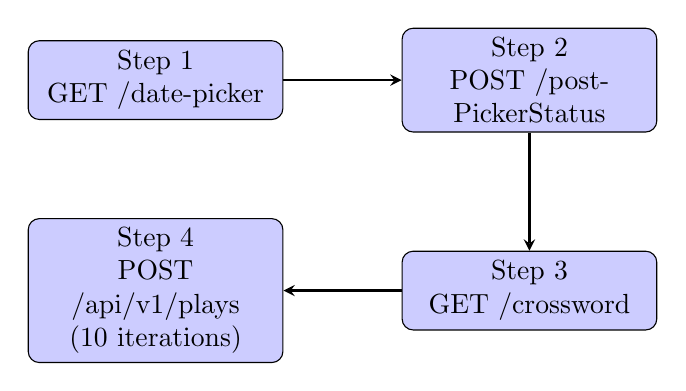
\begin{tikzpicture}[
        node distance=1.5cm,
        block/.style={rectangle, draw, fill=blue!20, text width=3cm, text centered, rounded corners, minimum height=1cm},
        arrow/.style={thick,->,>=stealth}
    ]
        \node[block] (step1) {Step 1\\GET /date-picker};
        \node[block, right=of step1] (step2) {Step 2\\POST /postPickerStatus};
        \node[block, below=of step2] (step3) {Step 3\\GET /crossword};
        \node[block, left=of step3] (step4) {Step 4\\POST /api/v1/plays\\(10 iterations)};
        
        \draw[arrow] (step1) -- (step2);
        \draw[arrow] (step2) -- (step3);
        \draw[arrow] (step3) -- (step4);
    \end{tikzpicture}
    \end{center}
    
    \vspace{0.5cm}
    \textbf{Simulates complete user journey:} Opening puzzle picker $\rightarrow$ Selecting puzzle $\rightarrow$ Playing the crossword
\end{frame}

\begin{frame}{Step 1: Date Picker Page}
    \textbf{Endpoint:} \texttt{GET /date-picker}
    
    \vspace{0.3cm}
    \textbf{Purpose:}
    \begin{itemize}
        \item Fetches the puzzle date picker HTML page
        \item Extracts \texttt{loadToken} from embedded JSON params
        \item Token required for all subsequent API calls
    \end{itemize}
    
    \vspace{0.3cm}
    \textbf{Parameters:}
    \begin{itemize}
        \item \texttt{set} - Puzzle series identifier
        \item \texttt{uid} - User identifier (random or fixed)
    \end{itemize}
    
    \vspace{0.3cm}
    \textbf{V3 Extension:} Also fetches CDN resources:
    \begin{itemize}
        \item \texttt{date-picker-min.css}, \texttt{picker-min.js}
        \item Font Awesome CSS and WOFF2 fonts
    \end{itemize}
\end{frame}

\begin{frame}[fragile]{Step 2: Post Picker Status}
    \textbf{Endpoint:} \texttt{POST /postPickerStatus}
    
    \vspace{0.3cm}
    \textbf{Purpose:}
    \begin{itemize}
        \item Notifies server that user is viewing the picker
        \item Validates the \texttt{loadToken}
        \item Records ad duration and verification status
    \end{itemize}
    
    \vspace{0.3cm}
    \textbf{Request Body:}
    \begin{lstlisting}[language=java]
{
    "loadToken": "<from step1>",
    "isVerified": true,
    "adDuration": 0,
    "reason": "displaying puzzle picker"
}
    \end{lstlisting}
\end{frame}

\begin{frame}{Step 3: Load Crossword}
    \textbf{Endpoint:} \texttt{GET /crossword}
    
    \vspace{0.3cm}
    \textbf{Purpose:}
    \begin{itemize}
        \item Loads the actual crossword puzzle page
        \item Extracts puzzle parameters and \texttt{playId}
        \item Uses hardcoded puzzle ID for consistent testing
    \end{itemize}
    
    \vspace{0.3cm}
    \textbf{Parameters:}
    \begin{itemize}
        \item \texttt{id} - Puzzle identifier
        \item \texttt{set}, \texttt{picker}, \texttt{uid}, \texttt{loadToken}
    \end{itemize}
    
    \vspace{0.3cm}
    \textbf{V3 Extension:} Also fetches:
    \begin{itemize}
        \item \texttt{crossword-player-min.css}
        \item \texttt{c-min.js} (crossword player script)
    \end{itemize}
\end{frame}

\begin{frame}{Step 4: Simulate Gameplay}
    \textbf{Endpoint:} \texttt{POST /api/v1/plays} (10 iterations)
    
    \vspace{0.3cm}
    \textbf{Purpose:}
    \begin{itemize}
        \item Simulates user solving the puzzle
        \item Sends state updates with progress
    \end{itemize}
    
    \vspace{0.3cm}
    \textbf{Play States:}
    \begin{enumerate}
        \item \textbf{playState=1}: Game started
        \item \textbf{playState=2} (iterations 2-9): In progress with mutations
        \item \textbf{playState=4}: Game completed
    \end{enumerate}
    
    \vspace{0.3cm}
    \textbf{State Management:}
    \begin{itemize}
        \item \texttt{primaryState}: Current letter entries
        \item \texttt{secondaryState}: Fill status bitmap
        \item Random mutations simulate real user behavior
    \end{itemize}
\end{frame}

%=============================================================================
\section{Why Java? Technology Choices}
%=============================================================================

\begin{frame}{Why Java Over Python?}
    \textbf{Performance Advantages:}
    \begin{itemize}
        \item \textbf{True multithreading} - No GIL limitations
        \item \textbf{Connection pooling} via OkHttp for efficient HTTP
        \item \textbf{Lower memory footprint} per thread
        \item \textbf{Predictable latency} - JIT compilation benefits
    \end{itemize}
    
    \vspace{0.5cm}
    \textbf{Scalability:}
    \begin{itemize}
        \item Handle higher RPS (requests per second)
        \item More accurate wave-based timing
        \item Better suited for long-running load tests
    \end{itemize}
\end{frame}

\begin{frame}{Technology Stack}
    \textbf{Build System:}
    \begin{itemize}
        \item \textbf{Maven} - Dependency management \& packaging
        \item \textbf{Java 17} - Modern language features
        \item \textbf{Maven Shade Plugin} - Uber JAR packaging
    \end{itemize}
    
    \vspace{0.3cm}
    \textbf{Key Dependencies:}
    \begin{table}[h]
    \centering
    \begin{tabular}{|l|l|l|}
    \hline
    \textbf{Library} & \textbf{Version} & \textbf{Purpose} \\
    \hline
    OkHttp & 4.12.0 & HTTP client with connection pooling \\
    \hline
    Gson & 2.10.1 & JSON parsing and serialization \\
    \hline
    OpenCSV & 5.9 & CSV result file generation \\
    \hline
    JCommander & 1.82 & CLI argument parsing \\
    \hline
    SLF4J & 2.0.9 & Logging framework \\
    \hline
    \end{tabular}
    \end{table}
\end{frame}

\begin{frame}[fragile]{OkHttp: Why This HTTP Client?}
    \textbf{Key Features:}
    \begin{itemize}
        \item \textbf{Connection pooling} - Reuses HTTP connections
        \item \textbf{HTTP/2 support} - Multiplexing for efficiency
        \item \textbf{Automatic retries} on connection failures
        \item \textbf{Configurable timeouts} (connect, read, write)
    \end{itemize}
    
    \vspace{0.5cm}
    \textbf{Configuration:}
    \begin{lstlisting}[language=java]
OkHttpClient client = new OkHttpClient.Builder()
    .connectTimeout(30, TimeUnit.SECONDS)
    .readTimeout(30, TimeUnit.SECONDS)
    .writeTimeout(30, TimeUnit.SECONDS)
    .build();
    \end{lstlisting}
\end{frame}

\begin{frame}[fragile]{Project Structure}
    \begin{columns}
    \column{0.5\textwidth}
    \textbf{Source Files:}
    \begin{itemize}
        \item \texttt{ApiFlowV2.java} - Main entry
        \item \texttt{ApiFlow.java} - HTTP flow logic
        \item \texttt{ApiFlowV3.java} - With CDN fetches
        \item \texttt{WaveExecutor.java} - RPS control
        \item \texttt{CsvResultWriter.java} - Output
        \item \texttt{HtmlReportWriter.java} - Dashboard
    \end{itemize}
    
    \column{0.5\textwidth}
    \textbf{Build Outputs:}
    \begin{itemize}
        \item \texttt{api-flow-v2.jar} - Standard flow
        \item \texttt{api-flow-v3.jar} - With CDN
    \end{itemize}
    
    \vspace{0.3cm}
    \textbf{Usage:}
    \begin{lstlisting}[basicstyle=\ttfamily\tiny]
java -jar api-flow-v2.jar \
  --rps 5 --duration 10 \
  --random-uid --html
    \end{lstlisting}
    \end{columns}
\end{frame}

%=============================================================================
\section{Dashboard \& Results}
%=============================================================================

\begin{frame}{HTML Dashboard: Overview}
    \textbf{Key Metrics Cards:}
    \begin{itemize}
        \item \textbf{Total Threads} - Number of test runs
        \item \textbf{Success Rate} - Percentage of successful flows
        \item \textbf{Avg Latency} - Mean response time
        \item \textbf{P95 Latency} - 95th percentile
        \item \textbf{Min / Max} - Latency range
    \end{itemize}
    
    \vspace{0.3cm}
    \textbf{Color Coding:}
    \begin{itemize}
        \item \textcolor{green}{\textbf{Green}} - Success rate $\geq$ 95\%
        \item \textcolor{orange}{\textbf{Yellow}} - Success rate 80-95\%
        \item \textcolor{red}{\textbf{Red}} - Success rate $<$ 80\%
    \end{itemize}
\end{frame}

\begin{frame}{Dashboard: Charts}
    \textbf{Three Visualization Types:}
    
    \vspace{0.3cm}
    \begin{enumerate}
        \item \textbf{Latency Distribution (Histogram)}
        \begin{itemize}
            \item Bucketed response times
            \item Shows distribution shape (normal vs skewed)
        \end{itemize}
        
        \vspace{0.2cm}
        \item \textbf{Per-Wave Average Latency}
        \begin{itemize}
            \item Line chart over time
            \item Detects performance degradation
        \end{itemize}
        
        \vspace{0.2cm}
        \item \textbf{Per-Thread Completion Time}
        \begin{itemize}
            \item Individual thread latencies
            \item Identifies outliers
        \end{itemize}
    \end{enumerate}
    
    \vspace{0.3cm}
    \textit{Charts use Chart.js with dark theme styling}
\end{frame}

\begin{frame}{Dashboard: Per-Wave Summary Table}
    \textbf{Columns:}
    \begin{table}[h]
    \centering
    \small
    \begin{tabular}{|l|p{5cm}|}
    \hline
    \textbf{Column} & \textbf{Description} \\
    \hline
    Wave & Wave number (1 wave = 1 second) \\
    \hline
    Success & Successful/Total threads in wave \\
    \hline
    Step1-4 Avg & Average latency per step \\
    \hline
    Total Avg & Sum of all step latencies \\
    \hline
    P95 & 95th percentile for the wave \\
    \hline
    \end{tabular}
    \end{table}
    
    \vspace{0.3cm}
    \textbf{Expandable Details:}
    \begin{itemize}
        \item Click wave to see individual thread results
        \item Includes UID, start time, per-step latencies
        \item Outliers highlighted ($>2\sigma$ from mean)
    \end{itemize}
\end{frame}

\begin{frame}{Dashboard: Error Summary}
    \textbf{Error Grouping:}
    \begin{itemize}
        \item Errors grouped by error message
        \item Sorted by count (most frequent first)
        \item Expandable to see affected threads
    \end{itemize}
    
    \vspace{0.3cm}
    \textbf{Error Details Table:}
    \begin{itemize}
        \item Wave and Thread numbers
        \item UID and Start Time
        \item Step latencies before failure
        \item Failed Step indicator
    \end{itemize}
    
    \vspace{0.3cm}
    \textbf{Visual Indicators:}
    \begin{itemize}
        \item Red left border for error sections
        \item Count badge with error frequency
        \item Monospace font for error messages
    \end{itemize}
\end{frame}

\begin{frame}{Dashboard Screenshot}
    \begin{center}
    % PLACEHOLDER: Add actual dashboard screenshot here
    \fbox{
        \parbox{0.8\textwidth}{
            \centering
            \vspace{3cm}
            \textbf{[Dashboard Screenshot Placeholder]}
            
            \vspace{0.3cm}
            \textit{Add screenshot of the HTML dashboard here}
            \vspace{3cm}
        }
    }
    \end{center}
\end{frame}

%=============================================================================
\section{Next Steps}
%=============================================================================

\begin{frame}{Summary \& Next Steps}
    \textbf{What We Covered:}
    \begin{itemize}
        \item 4-step API flow simulating user journey
        \item Java technology stack and library choices
        \item HTML dashboard format and metrics
    \end{itemize}
    
    \vspace{0.5cm}
    \textbf{Next Steps:}
    \begin{itemize}
        \item Add actual test results
        \item Include performance benchmarks
        \item Compare V2 vs V3 flow performance
        \item Add CDN latency breakdown analysis
    \end{itemize}
\end{frame}

\begin{frame}
    \begin{center}
    \Huge{Questions?}
    \end{center}
\end{frame}

\end{document}
